\documentclass[10pt]{article}
\usepackage[cp1251]{inputenc}
\usepackage[english]{babel}
\usepackage{url}
\usepackage{graphicx,DCCN2015_en}
\newcommand{\Rmnum}[1]{\expandafter\@slowromancap\romannumeral #1@}


\makeatletter
\c@page=1 % Number will be set by publisher.
          
\makeatother


% Proper title, should be and will be capitalized
\title{Low-priority Queue Fluctuations in Tandem of Queuing Systems under Cyclic Control with Prolongations}
\author{V.~M.~Kocheganov$^1$, A.~V.~Zorine$^1$}
\company{$^1$ Departament of Applied Probability Theory, N.~I.~Lobachevsky State University of Nizhny Novgorod, Nizhny Novgorod, Russia}
\email{kocheganov@gmail.com, zoav1602@gmail.com}


%%%%%%%%%%%%%%%%%%%%%%%%%%%%%%%%

\begin{document}

\maketitle

%%%%%%%%%%%%%%%%%%%%%%%%%%%%%%%%%%%%%%%%%%%%%%%%%%%%%%%%%%%%%%
\begin{abstract}
A tandem of queuing systems is considered. Each system has a high-priority input flow and a low-priority input flow which are conflicting. In the first system, the customers are serviced in the class of cyclic algorithms. The serviced high-priority customers are transferred from the first system to the second one  with random delays and become the high-priority input flow of the second system. In the second system, customers are serviced in the class of cyclic algorithms with prolongations. Low-priority customers are serviced when their number exceeds a threshold. A mathematical model is constructed in form of a multidimensional denumerable discrete-time Markov chain. The recurrent relations for partial probability generating functions for the low-priority queue in the second system are found.

\keywords{tandem of controlling queuing systems, cyclic algorithm with prolongations, conflict flows, multidimensional denumerable discrete-time Markov chain}
\end{abstract}
%%%%%%%%%%%%%%%%%%%%%%%%%%%%%%%%%%%%%%%%%%%%%%%%%%%%%%%%%%%%%%


\section{Introduction}
Conflict traffic flows control at a crossroad is one of the classical problem of queuing theory. The problem has been solved for different classes of algorithms: the class of algorithms with a cyclic fixed rhythm, with renewals ("with a loop") with dynamic priorities, etc. However, several (two in our case) consecutive crossroads are of great interest, because in a real life after car passed one highway intersection it finds itself at another one. In other words, output flow of the first intersection forms input flow of the second intersection. Hence, the second input flow no longer has simple probabilistic structure known a priori (for example, non-ordinary Poison process) and knowledge about service algorithm should be taken into account to deduce formation properties of the first output flow.

In [1] the problem of tandem of two crossroads was carried out and rigorous probabilistic model was built. At each of the intersections, in addition to the high priority flow, there was the traffic flow "in the perpendicular direction", with lower priority. The service of the flows on first intersection is supposed to be in the class of cyclic algorithms and in the of cyclic algorithms with prolongations on the second intersection. Over and above, vehicles could not turn from one conflict direction to another. In this paper we continue the study of described problem and deepen in low priority flow of the second intersection investigation.


\section{The setting of the problem}

This section contains statement of the problem according to []. First of all the tandem is presented as queuing system to give generic formulation while in the end of the section system of two consecutive crossroads is brought as simple example. More rigorous mathematical model is built in next section.

Consider queuing system of the following type:
\begin{figure}[h!]
   \centering
    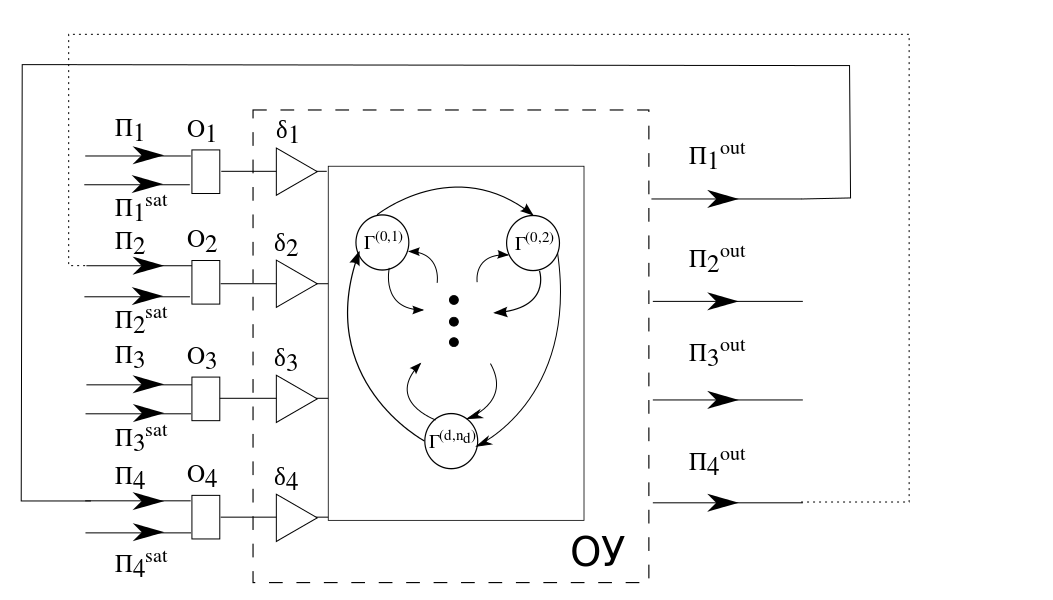
\includegraphics[width=\textwidth]{SystemScheme.png} % or {1.eps} in case of EPS format of the picture
    \caption {Structure scheme of queuing system}
    \label{pic1}
\end{figure}
There are four input flows of customers coming into the system with one server. Customers from input flow $\Pi_j$ arrive to corresponding queue with an unbounded capacity, $j \in \{1,2,3,4\}$. For $j \in \{1,2,3\}$ discipline of the queue $O_j$ is FIFI (First In First Out). In other words, the earlier customer came to system the earlier it is serviced. Disciplie of the queue $O_4$ is described below. Input flows $\Pi_1$ and $\Pi_3$ are generated by external environment, which has only one state. Each of these flows is a nonordinary Poisson process. Denote $\lambda_1$ and $\lambda_3$ the intensity for the bulk arrival for the flows $\Pi_1$ and $\Pi_3$ respectively. Generating function of customer number in the bulk of flow $\Pi_j$ is
\begin{equation}
f_j(z) = \sum_{\nu=1}^{\infty} p_{\nu}^{(j)} z ^{\nu}, \quad j\in \{1,3\},
\label{GeneratingFunc}
\end{equation}
assuming it is finite for any $z\in \mathbb{C}$ such as $|z|<(1+\varepsilon)$, $\varepsilon>0$. Quantity $p_{\nu}^{(j)}$ is probability of event that customers number in a bulk of flow $\Pi_j$ is exactly $\nu$. Being serviced $\Pi_1$ customers come back to the system as $\Pi_4$ customers. $\Pi_4$ customers in turn after service come back to the system as $\Pi_2$ ones. Flows $\Pi_2$ and $\Pi_3$ are conflicting in the sense that customers arriving from different sources cannot be served simultaneously in the same queuing system. This means that the problem cannot be reduced to a corresponding problem with fewer input flows by merging the flows together.

Given positive integers $d$, $n_0$, $n_1$, $\ldots$, $n_d$, we introduce a finite set $\Gamma=\{\Gamma^{(k,r)} \colon k=0,1,\ldots,d; r=1,2,\ldots n_k\}$ of states in which server can be. At each state $\Gamma^{(k,r)}$ sever stays during time $T^{(k,r)}$. Define sets $\Gamma^{\mathrm{I}}$, $\Gamma^{\mathrm{II}}$, $\Gamma^{\mathrm{III}}$ and $\Gamma^{\mathrm{IV}}$ as follows. 
In state $\gamma \in \Gamma^{\mathrm{I}}$ only customers of queues $O_1$, $O_2$ and $O_4$ are serviced.
In state $\gamma \in \Gamma^{\mathrm{II}}$ only customers of queues $O_2$ and $O_4$ are serviced.
In state $\gamma \in \Gamma^{\mathrm{III}}$ only customers of queues$O_1$, $O_3$ and $O_4$ are serviced.
In state $\gamma \in \Gamma^{\mathrm{IV}}$ only customers of queues$O_3$ and $O_4$ are serviced.
The set $\Gamma$ defines as union $\Gamma = \Gamma^{\mathrm{I}} \cup \Gamma^{\mathrm{II}} \cup \Gamma^{\mathrm{III}} \cup \Gamma^{\mathrm{III}}$ disjoint sets. We will also need following sets in the future ${}^1\Gamma=\Gamma^{\mathrm{I}} \cup \Gamma^{\mathrm{III}}$, 
${}^2\Gamma=\Gamma^{\mathrm{I}} \cup \Gamma^{\mathrm{II}}$,
${}^3\Gamma=\Gamma^{\mathrm{III}} \cup \Gamma^{\mathrm{IV}}$. 

Server changes its state according following rule. We will call the set $C_k = \{\Gamma^{(k,r)} \colon r=1,2,\ldots n_k\}$  $k$th cycle, $k=1$, $2$, $\ldots$, $d$ (Pic. \ref{GraphScheme}). When $k=0$ state of the form 
$\Gamma^{(0,r)}$ we will call prolongation state, $r=1$, $2$, $\ldots$, $n_0$. Denote $r \oplus_k 1 = r+1$ for $r<n_k$ and $r \oplus_k 1 = 1$ while $r=n_k$, $k = 0$, $1$, $\ldots$, $d$. In cycle $C_k$ we select subsets $C_k^{\mathrm{O}}$ input, $C_k^{\mathrm{I}}$ output and $C_k^{\mathrm{N}} = C_k \setminus (C_k^{\mathrm{O}} \cup C_k^{\mathrm{I}})$ neutral states. 
Then  after server was in state $\Gamma^{(k,r)} \in C_k\setminus C_k^{\mathrm{O}}$ it switches to the state $\Gamma^{(k,r \oplus_k 1)}$ of the same cycle $C_k$. 
After state $\Gamma^{(k,r)}$ in $C_k^{\mathrm{O}}$ server switches to the state $\Gamma^{(k,r \oplus_k 1)}$, if number of customers in the queue $O_3$ in switching moment greater than predetermined threshold $L$. In other case,  that is if number of customers in the queue $O_3$ lesser or equal $L$, then new state is prolongation state $\Gamma^{(0,r_1)}$, where 
$r_1=h_1(\Gamma^{(k,r)})$ and
$h_1(\cdot)$~--- given mapping of the set 
$\bigcup\limits_{k=1}^d C_k^{\mathrm{O}}$ on $\{1,2,\ldots, n_0\}$. 
After state $\Gamma^{(0,r)}$ the state of the same type $\Gamma^{(0,r_2)}$ is chosen, if number of customers in queue $O_3$ is lesser or equal $L$, where $r_2=h_2(r)$ and $h_2(\cdot)$~--- given mapping of the 
set $\{1,2, \ldots, n_0\}$ on itself; in other case state of the form $\Gamma^{(k,r_3)} \in C_k^{\mathrm{I}}$ is on, where $\Gamma^{(k,r_3)}=h_3(r)$ and $h_3(\cdot)$~--- given mapping $\{1,2, \ldots, n_0\}$ on the set  $\bigcup\limits_{k=1}^d C_k^{\mathrm{I}}$. We assume that all prolongation states $\Gamma^{(0,r)}$ belong to the set ${}^2 \Gamma$, and  relations $C_k^\mathrm{O}\subset {}^2 \Gamma$ and $C_k^\mathrm{I}\subset {}^3 \Gamma$ are hold. We also assume that all the cycles have exactly one input and output state. And last assumption is that all the prolongation vertices form one cycle, that is we can put $h_2(r)=r\oplus_0 1$.

More formally server changes its states according to the following rule:
\begin{equation}
h(\Gamma^{(k,r)},y) = 
\begin{cases}
\Gamma^{(k,r \oplus_k 1)},& \quad \text{ if } (\Gamma^{(k,r)}\in C_k\setminus C_k^{\mathrm{O}}) \text{ or } (\Gamma^{(k,r)}\in C_k^{\mathrm{O}} \text{ \& } y>L);\\
%\Gamma^{(k,r \oplus_k 1)},& \quad \text{ if } \Gamma^{(k,r)}\in C_k^{\mathrm{O}} \text{ and } y>L;\\
\Gamma^{(0,h_1(\Gamma^{(k,r)}))},& \quad \text{ if } \Gamma^{(k,r)}\in C_k^{\mathrm{O}} \text{ and } y\leqslant L;\\
\Gamma^{(0,r \oplus_0 1)},& \quad \text{ if } k=0 \text{ and } y\leqslant L;\\
h_3(r),& \quad \text{ if } k=0 \text{ and } y > L.
\end{cases}
\label{hLaw}
\end{equation}

In general service durations of different customers can be dependent and have different distributions. That is why instead of classic approach  which specifies distributions of every particular customer, saturation flows will be used. Such a flow $\Pi^{\mathrm{\text{sat}}}_j$, $j \in \{1,2,3,4\}$, 
is defined as virtual output flow given maximum loading of the server, and for $j\in \{1, 2, 3\}$ given also maximum loading of the corresponding queue. Saturation flow $\Pi^{\mathrm{\text{sat}}}_j$, $j\in \{1,2,3\}$ 
contains non-random number of customers $\ell_{k,r,j}$, serviced during $T^{(k,r)}$, if server's state is $\Gamma^{(k,r)}$. Let $\mathbb{Z}_+$~--- be the set of non-negative integer numbers. Then given the fact, that queue $O_4$ contains $x \in \mathbb{Z}_+$ customers, saturation flow $\Pi^{\mathrm{\text{sat}}}_4$ is determined to contain all the $x$ customers.
Finally in the state $\Gamma^{(k,r)}$ every customer from queue $O_4$ with probability $p_{k,r}$ and independently of others ends servicing and come to queue $O_2$ of the flow $\Pi_2$. The customer of queue $O_4$ stay on up to the next round with probability $1-p_{k,r}$. On next round the picture is the same.

As we mentioned earlier in the end of the section we introduce real-life example of defined queuing system: tandem of two consecutive crossroads (Fig. \ref{crossroads}). 
\begin{figure}[h!]
   \centering
    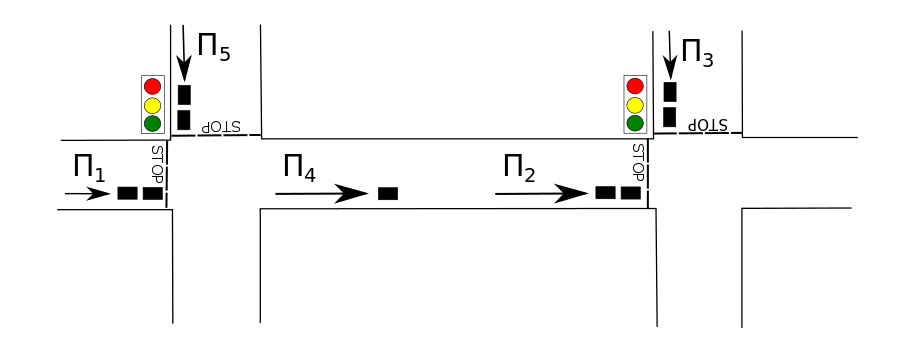
\includegraphics[width=\textwidth]{Crossroads.png} % or {1.eps} in case of EPS format of the picture
    \caption {Example: crossroads tandem}
    \label{pic1}
\end{figure}
Flows of arriving cars play role of customer flows formed by external environment: conflicting flows $\Pi_1$ and $\Pi_5$ on the first crossroad; flow $\Pi_3$ on the second. Every car from flow $\Pi_1$, after passing first road intersection, comes to the queue $O_4$ of the flow $\Pi_4$. Whereupon the car arrives to the next road intersection with some probability ($p_{k,r}$ for the state $\Gamma^{(k,r)}$) or does not have time to do so and stays for another round. In case it has time it comes in queue $O_2$ and waits it's turn to pass it. Such system is an instance of more general queuing model described above.



The full source text using \TeX{} as well as all auxiliary
materials, namely,
\begin{itemize}
  \item .tex file,
  \item pictures in .pdf (or .eps) format (if available),
  \item the paper in pdf format
\end{itemize}
have to be submitted as a zip-archive.

The name of the archive should be
\textbf{Surname1\_Surname2\_Surname3.zip}.

\section{Font}

Type the text of the paper in 10 points, regular. Each
paragraph is to be indented 5~mm, and their intervals must be 0
points before and after.

\section{Mathematical formulae and references}

To make references to mathematical expressions, it is
recommended to use \LaTeX{} mechanism. For example, the formula
given below
\begin{equation}
\label{eq:1}
P(n,t)=\frac{\partial^n B(t)}{\partial t^n}
\end{equation}
can be referred as \eqref{eq:1}.

\section{Theorems and proofs}

Theorems are defined like follows
\begin{thm}\label{thm1}
Text of the theorem.
\end{thm}

\begin{proof}
Proof of Theorem \ref{thm1}. If using such reference, you need
to recompile your paper with \LaTeX{} twice.
\end{proof}


\section{Figures and tables}

Figures should be provided in PDF or EPS format. Raster pictures have
to be made with maximal resolution (minimal 300 dots per inch).

\begin{figure}[h!]
   \centering
    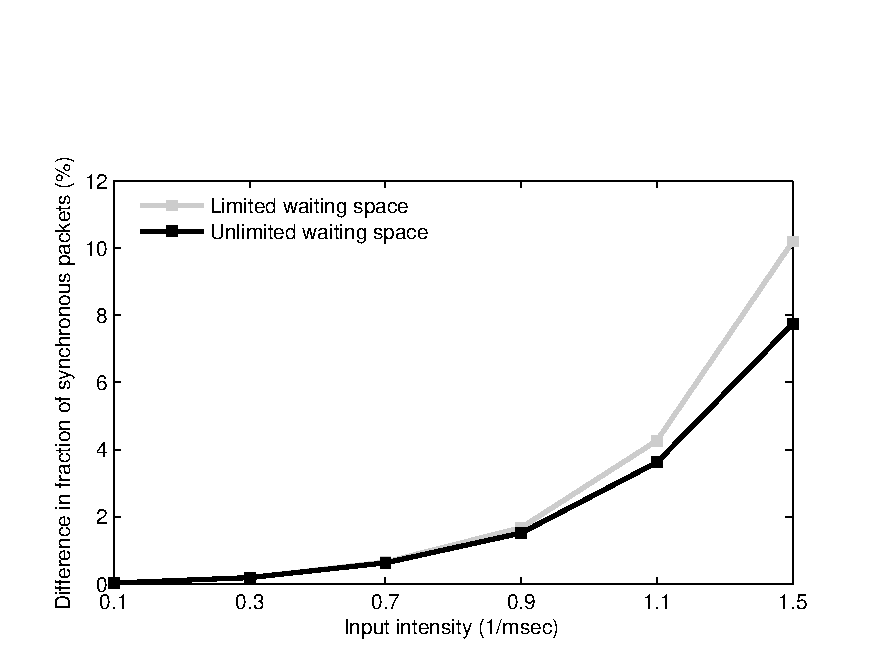
\includegraphics[width=\textwidth]{1.pdf} % or {1.eps} in case of EPS format of the picture
    \caption {Difference in fractions of synchronous packets for $W=16$.}
    \label{pic1}
\end{figure}

\begin{table}[h!]\begin{center}
\label{tab}
\begin{tabular}{|c||c|c|c||c||c|c|c|}\hline
  Parameter & T & E & $\Delta$, \% & Parameter & T & E & $\Delta$, \% \\ \hline \hline
  $\rho_{1}^{(1)}$ & 0,187 & 0,194 & 3,7 &  $\rho_{1}^{(2)}$ & 0,127 & 0,120 & 5,6 \\ \hline
  $\rho_{2}^{(1)}$ & 0,073 & 0,072 & 1,4 &  $\rho_{2}^{(2)}$ & 0,052 & 0,053 & 1,9 \\ \hline
  $\rho_{3}^{(1)}$ & 0,148 & 0,147 & 0,7 &  $\rho_{3}^{(2)}$ & 0,103 & 0,103 & 0,0 \\ \hline
  $\rho_{4}^{(1)}$ & 0,036 & 0,036 & 0,0 &  $\rho_{4}^{(2)}$ & 0,026 & 0,027 & 3,7 \\ \hline \hline
  $C^{(1)}$ & 0,479 & 0,476 & 0,6 & $C^{(2)}$ & 0,656 & 0,640 & 2,5 \\ \hline \hline
  $C_{1}^{*}$ & 0,341 & 0,339 & 0,6 & $C_{3}^{*}$ & 0,323 & 0,329 & 1,8 \\ \hline
  $C_{2}^{*}$ & 0,296 & 0,298 & 0,7 & $C_{4}^{*}$ & 0,286 & 0,286 & 0,0 \\ \hline
\end{tabular}\caption{Comparison of system parameters.}
\end{center}\end{table}

The figures and tables must be numbered, have a self-contained
caption and referred in the main text. Figure and table
captions are placed below the object and centered. Also, avoid
placing figures and tables before their first mention in the
text. Use the abbreviation "Fig." even at the beginning of a
sentence.

The authors are recommended not to use characters smaller than
9 point in figures. Do not use abbreviations in the titles
unless they are unavoidable.


\section{Conclusion}

Place a full list of references \cite{Bianchi00, VL02, neuts, GPSS, url} at the end of the paper. List
the references according to the order of their appearance in
the text.

%{\bf Acknowledgments.}

\begin{thebibliography}{99}
\bibitem{Bianchi00}  %% citation code
Bianchi G. Performance Analysis of the IEEE 802.11 Distributed
Coordination Function ~// IEEE Journal on Selected Areas in
Communications. 2000. V. 18. P.~535-547.

\bibitem{VL02} Vishnevsky V.~M., Lyakhov A.~I. IEEE 802.11
    Wireless LAN: Saturation Throughput Analysis with Seizing
    Effect Consideration
// Cluster Computing. 2002. V. 5. P. 133-144.

\bibitem{neuts} Neuts M.~F.  Structured Stochastic
    Matrices of M/G/1 Type and Their Applications. Marcel
    Dekker, New York, 1989.

\bibitem{GPSS} Schriber T.~J. Simulation using GPSS. John
    Wiley \& Sons, 1974.
    
\bibitem{url} National Center for Biotechnology Information, \url{http://www.ncbi.nlm.nih.gov}

\end{thebibliography}

\end{document}
